\chapter{基于树形条件随机场的高效依存句法分析}\label{cha:dep-crf}

本章深入详细的比较了与当前最佳的Biaffine Parser所采用的局部训练相比,基于全局树形条件随机场训练的方法的效果,并首次提出了在神经依存句法分析器上应用一个二阶树形条件随机场的拓展.
由于高复杂度和低效一直以来都是困扰树形条件随机场的广泛应用的一个重要原因,因此我们提出了一个能够高效批次化Inside算法和Eisner算法的方法,来支持树形条件随机场在GPU上的大规模张量并行计算.
并且,我们还通过反向传播机制,避免了复杂Outside算法的计算.
我们在13个语言的27个数据集上进行了实验,实验结果和分析表明,在深度学习时代之前的技术,诸如结构化学习(全局树形条件随机场损失函数)和高阶建模仍然是有益的,并且可以进一步在最好的Biaffine Parser的基础上提升性能,尤其是在局部标注的场景下.

\section{引言}
\input{figures/dep-example.tex}
依存句法分析任务是NLP领域的一个基础性任务,由于其简洁性,以及可以方便的在多语言上获得句法和语义信息的特性,目前在这一任务上已经有了大量的研究. 如图\ref{fig:dep-tree-example}所示,给定一个句子$\boldsymbol{x}=w_0w_1\cdots w_n$,一棵依存树被定义为$\boldsymbol{y}=\{(i,j,l),0\le i \le n,1 \le j \le n,l \in \mathcal{L}\}$,其中$(i,j,l)$是一条从头(head)$w_i$到修饰词(modifier)$w_j$的弧,弧的标签为$l \in \mathcal{L}$. 目前在依存句法分析任务上有两个主流方法,分别是基于转移(transition-based)的方法,和基于图(graph-based)的方法,这里我们的方法主要关注于基于图的解析方式.

在深度学习时代之前,基于图的解析依赖于很多手工特征的设计,比如词性、前缀、后缀等等.
与神经网络方法相比,以前的方法有两个显著的不同.
首先,对于非神经网络方法而言,结构化学习(结构化学习)是不可或缺的,即训练时需要显式地建模树结构的约束.
通常此类方法采用的是max-margin训练算法,首先用当前模型训练一棵分值最高的树,然后更新模型参数,以保证正确的树的分值要高于预测树.

第二个显著的区别在于高阶特征的使用. 高阶特征为模型带来了显著的提升.
基础的一阶模型将句法树的分值分解为若干条独立的弧的分值\cite{mcdonald-etal-2005-online}. 后续的工作进一步引入了二阶依存弧对对分值,比如邻接兄弟\cite{mcdonald-pereira-2006-online}和祖父-父亲-孩子这样的弧对\cite{carreras-2007-experiments,koo-collins-2010-efficient},这些高阶扩展都带来了模型性能的显著提升\footnote{三阶和四阶模型的提升不大,这可能是由于特征稀疏的问题导致的\cite{koo-collins-2010-efficient,ma-zhao-2012-fourth}.}. 但是这些高阶模型需要引入更复杂的解码算法,导致了模型更加低效.


相比之下,基于图的神经网络依存句法分析器的发展呈现出相反的趋势.
\cite{pei-etal-2015-effective}提出利用前馈神经网络来自动学习\cite{chen-manning-2014-fast}的若干特征组合,并计算子树得分.
他们的工作表明引入二阶邻接兄弟子树的分值显著提高了性能。
随后,\cite{wang-chang-2016-graph}和\cite{kiperwasser-goldberg-2016-simple}都建议使用双向LSTM作为编码器和,以及在一阶模型中利用minus-feature来对单条弧打分.
这三个代表性方法都采用了全局的max-margin方法.
\cite{Timothy-d17-biaffine}提出了一种强大而高效的Biaffine Parser,并在各种数据集和语言上获得了最先进的精度.
Biaffine Parser也是一阶的,通过对每个词进行局部头选择(head selection)的方式\cite{zhang-etal-2017-dependency-parsing},采用了更简单、更有效的非结构化训练方法.

基于这些对比,我们尝试在基于图的解析器的基础上,将前深度学习时代的一些方法与神经网络模型做一下连接.
这里要解决的\textbf{第一个问题}是:
\emph{以前的一些技术,比如结构化学习和高阶建模,能够进一步提升当前最佳的解析器Biaffine Parser的性能吗\footnote{
        尽管最近的一些工作汇报了相比Biaffin Parser更高的性能,但是都引入了一些外部资源,比如大规模语言模型的上下文词表示. 在相同网络和相同实验设置的场景下,这些工作的结果都是相近的.
    },如果可以,他们在哪些方面是有用的?}

对于结构化学习而言,相比max-margin方法,我们采用更复杂且更不常用的TreeCRF.
主要原因有两方面.
首先,概率分布估计一直是当前数据驱动的NLP方法的一个核心的问题\cite{le-zuidema-2014-inside}.
如果将解析器的输出应用到更高层的任务,一棵句法树的概率$p(\boldsymbol{y}\mid\boldsymbol{x})$比没有上下边界的分值$s (\boldsymbol{x},\boldsymbol{y})$一般而言要更加有用.
其次,边缘概率是一种理论上比较可靠的方法来评估模型输出子树的置信度,可以用于最小贝叶斯风险(MBR)解码\cite{smith-smith-2007-probabilistic},并且已经被证明了对于词级别基于局部标注句法树的主动学习(active learning)\cite{li-etal-2016-active}很有用.

尽管很有用,但是TreeCRF不如max-margin那么留下,其中一个原因是由于inside-outside算法的高复杂度,尤其是outside算法.
据我们所知,所有现存的模型都是在CPU上运算inside-outside算法.
而由于CPU/GPU巨大的效率差异,这一低效的问题在深度学习时代变得更加严重.
这就引发了\textbf{第二个问题}:
\emph{我们是否能够批次化inside-outside算法,并且直接在GPU上进行计算?}
如果这样的话,我们就能够利用诸如PyTorch这样的高效深度学习张量库来进行计算,并且将高效的TreeCRF应用到更多的场景\cite{cai-etal-2017-crf,le-zuidema-2014-inside}.

总体而言,针对上面的两个问题,我们做了下面的几个贡献:
\begin{itemize}%[leftmargin=10pt,topsep=3pt,itemsep=1pt,partopsep=1pt]
    \item 我们第一次提出了将二阶TreeCRF应用到神经依存句法分析中.
          我们还提出了一个高效的Triaffine结构来对于二阶子树打分.
    \item 我们提出通过GPU上大规模的并行张量计算来批次化inside算法,来进行更高效的TreeCRF损失函数的计算.
          我们表明复杂的outside算法对于梯度和边缘概率的计算而言已不再必须,相应的可以用高效的反向传播代替.
    \item 我们在13个语言的27个树库上进行了实验.
          结果和分析都表明,深度学习时代的,结构化学习和高阶建模在许多方面对当前最好的Biaffine Parser仍然是有用的.
\end{itemize}

\section{基线模型}
\label{sec:basic_model}

我们复现了当前最好的Biaffine Parser\cite{Timothy-d17-biaffine},并在两方面对其做了修改:1) 用CharLSTM代替原来的词性embedding,2) 用一阶Eisner算法\cite{eisner-2000-iwptbook}代替原来的MST算法来进行投影树解码.

\subsection{打分方法}
图~\ref{fig:dep-framework}展示了我们的打分架构,一共由四个部分组成.

\textbf{输入向量.}
第$i$个输入向量可以分为两部分:词向量,以及词$w_i$的CharLSTM表示向量.
\begin{equation}
    \label{eq:input}
    \mathbf{e}_i=\mathrm{emb}({w_i}) \oplus \mathrm{CharLSTM}(w_i)
\end{equation}
其中$\mathrm{CharLSTM}(w_i)$是由先将$w_i$输入到一个双向LSTM,然后拼接两个最后的隐向量获得\cite{lample-etal-2016-neural}.
我们发现用$\mathrm{CharLSTM}(w_i)$替换原有的词性embedding会带来稳定的提升,并且也简化了实验流程,尤其是对于多语言实验恶言,无需再用到词性标注器来额外生成输入句子的词性.

\noindent\textbf{双向LSTM编码器.}
为了编码句子级别的上下文,解析器对输入$\mathbf{e}_0 \dots \mathbf{e}_n$应用了三层双.
顶层双向LSTM的第$i$个词的输出向量被表示为$\mathbf{h}_i$.

\noindent\textbf{MLP特征提取层.}
两个共享的MLP层被应用到了$\mathbf{h}_i$上来获取相应的低维向量,通过这种方式只保留句法相关的信息
\begin{equation}
    \label{mlp-arc}
    \mathbf{r}_i^{h}; \mathbf{r}_i^{m} =\mathrm{MLP}^{h/m} \left( \mathbf{h}_i \right)
\end{equation}
其中$\mathbf{r}_i^{h}$和$\mathbf{r}_i^{m}$是词$w_i$分别作为一条弧的头和修饰词的表示.

\noindent\textbf{Biaffine打分器.}
\cite{Timothy-d17-biaffine}首次提出通过biaffine attention计算一条依存弧$i \rightarrow j$的分值
\begin{equation} \label{eq:biaffine}
    s(i,j) =  \left[
        \begin{array}{c}
            \mathbf{r}_{j}^{m} \\
            1
        \end{array}
        \right]^\mathrm{T}
    \mathbf{W}^\textit{biaffine}  \mathbf{r}_{i}^{h}
\end{equation}
其中$\mathbf{W}^\textit{biaffine} \in \mathbb{R}^{d \times d}$.
这种计算方式在GPU上进行尤其高效.

\begin{figure}[tb]
    \centering
    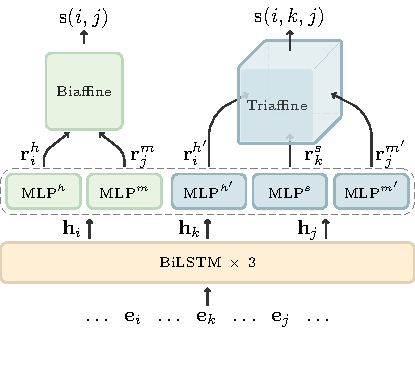
\includegraphics[scale=1.5]{figures/framework.pdf}
    \caption{带二阶扩展的打分架构.}
    \label{fig:dep-framework}
\end{figure}

\subsection{局部词级别训练损失}
Biaffine Parser采用了一个简单的词级别非结构化损失函数,试着对每个词独立最大化正确头的局部概率.
在一个训练实例中,对于一个正确的头-依赖对$(w_i, w_j$),其对应的交叉熵损失为
\begin{equation} \label{eq:biaffine-loss}
    \mathit{L}(i,j) = -\log{\frac{e^{s(i,j)}}{\sum_{0 \le k \le n} e^{s(k,j)}}}
\end{equation}
换句话说,模型的训练是基于一个简单的头选择目标,最终所有词的损失都被累加起来,而没有考虑任何树结构的约束.

\subsection{解码}
有了所有依存弧的分值,我们采用复杂度为$O(n^3)$的一阶Eisner算法来寻找最优的句法树.
\begin{equation}
    \label{eq:map-decoding}
    {\boldsymbol{y}}^* = \arg\max_{\boldsymbol{y}} \left[ s(\boldsymbol{x},\boldsymbol{y}) \equiv
        \sum_{i \rightarrow j \in \boldsymbol{y}}{s(i,j)} \right]
\end{equation}

\subsection{依存标签处理}
Biaffine Parser将骨干树的搜索和依存弧标签标注视为两个独立的任务.
这里为了方便我们采取了相同的策略. 具体细节可以参考\cite{Timothy-d17-biaffine}.

\begin{figure}[tb]
    \centering
    \begin{subfigure}[b]{0.45\textwidth}
        \centering
        \includegraphics[scale=1.5]{figures/scoring-part/a.pdf}
        \caption{单弧}
        \label{fig:scoring-part-a}
    \end{subfigure}
    \begin{subfigure}[b]{0.45\textwidth}
        \centering
        \includegraphics[scale=1.5]{figures/scoring-part/b.pdf}
        \caption{邻接兄弟}
        \label{fig:scoring-part-b}
    \end{subfigure}
    \caption{两种打分的子树结构.}
    \label{fig:scoring-part}
\end{figure}



\section{二阶TreeCRF}\label{2o-tree-crf}
我们从两方面极大地拓展来Biaffine Parser:
使用概率TreeCRF来进行结构化训练,以及显式引入高阶子树地分值.

具体地我们在基本的一阶模型的基础上引入了二阶邻接子树的分值:\footnote{
    我们还可以进一步扩展,引入祖父-父亲-孩子的子树分值,然后基于\cite{koo-collins-2010-efficient}提出的$O(n^4)$的Viterbi算法解码.
    这里我们留待作为未来的工作.
}
\begin{equation}\label{eq:score-definition-2o}
    s(\boldsymbol{x}, \boldsymbol{y}) = \sum_{i\rightarrow j \in \boldsymbol{y}}s(i,j) + \sum_{
        %\begin{array}{c}
        i\rightarrow \{k,j\} \in \boldsymbol{y} %\
        %  i\rightarrow k \in \boldsymbol{y}
        %\end{array}
    } s(i,k,j)
\end{equation}
其中$k$和$j$是$i$的两个相邻的孩子,并且满足$i < k < j$或者$j < k < i$.
图\ref{fig:scoring-part}展示了两种我们要打分的子树结构.

作为一个概率模型,TreeCRF以下面的方式计算一棵树的条件概率
\begin{equation}\label{eq:prob-labeled}
    \begin{split}
        & p(\boldsymbol{y}\mid\boldsymbol{x})  = \frac{e^{s(\boldsymbol{x},\boldsymbol{y})}}{Z(\boldsymbol{x}) \equiv \sum_{\boldsymbol{y'} \in \mathcal{Y}(\boldsymbol{x})} {e^{s(\boldsymbol{x},\boldsymbol{y'})}}}
    \end{split}
\end{equation}
其中$\mathcal{Y}(\boldsymbol{x})$是输入句子$\boldsymbol{x}$对应所有合法的句法树,$Z(\boldsymbol{x})$通常被成为normalization/partition term.

训练时,TreeCRF应用了下面的损失函数来最大化给定$\boldsymbol{x}$正确句法树$\boldsymbol{y}$的条件概率.
\begin{equation}\label{eq:training-loss-treecrf}
    \begin{split}
        \mathit{L}(\boldsymbol{x},\boldsymbol{y}) &= -\log p(\boldsymbol{y}\mid\boldsymbol{x})  \\
        &= - s(\boldsymbol{x}, \boldsymbol{y}) + \log Z(\boldsymbol{x})
    \end{split}
\end{equation}

\begin{figure}[tb]
    \centering
    \begin{subfigure}[b]{\textwidth}
        \begin{minipage}{\textwidth}
            \centering
            \includegraphics[scale=1.35]{figures/eisner-2o/a.pdf}
            \label{fig:eisner-2o-a}
        \end{minipage}
    \end{subfigure}
    \begin{subfigure}[b]{\textwidth}
        \begin{minipage}{\textwidth}
            \centering
            \includegraphics[scale=1.35]{figures/eisner-2o/b.pdf}
            \label{fig:eisner-2o-b}
        \end{minipage}
    \end{subfigure}
    \begin{subfigure}[b]{\textwidth}
        \begin{minipage}{\textwidth}
            \centering
            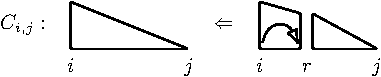
\includegraphics[scale=1.35]{figures/eisner-2o/c.pdf}
            \label{fig:eisner-2o-c}
        \end{minipage}
    \end{subfigure}
    \caption{基于自底向上动态规划的二阶Inside算法图示.}
    \label{fig:eisner-2o}
    % \vspace{-5pt}
\end{figure}

\subsection{二阶子树打分}
未来避免对原有打分架构有大的改动,我们采用来一个直接的扩展来获得邻接子树的分值.
首先,我们用三个额外的MLP层来进行和Biaffine所需要的类似的特征提取
\begin{equation}
    \label{mlp-sib}
    \mathbf{r}_i^{h'}; \mathbf{r}_i^{s}; \mathbf{r}_i^{m'} =\mathrm{MLP}^{h'/s/m'} \left( \mathbf{h}_i \right)
\end{equation}
$\mathbf{r}_i^{h'}; \mathbf{r}_i^{s}; \mathbf{r}_i^{m'}$是词$w_i$分别作为头,兄弟,和依赖对应的表示.\footnote{
    另一种方式是重用一阶部分头和依赖的表示,但是我们的前置实验表明这种方法的结果要更差一点
}

然后,我们提出来一个对biaffine equation自然的扩展,triaffine结构,来通过上述的三个向量计算分值\footnote{
    我们同样尝试了\cite{wang-etal-2019-second}的方法,他们用了三个biaffine操作来模拟三个输入向量的交互,但是这种方法的结果相对要差一点.
    篇幅限制我们省略了相应结果的汇报.
}
\begin{equation} \label{eq:triaffine}
    s(i,k,j) =
    \left[
        \begin{array}{c}
            \mathbf{r}_{k}^{s} \\
            1
        \end{array}
        \right]^\mathrm{T}
    {\mathbf{r}_{i}^{h'}}^\mathrm{T}
    \mathbf{W}^\textit{triaffine}
    \left[
        \begin{array}{c}
            \mathbf{r}_{j}^{m'} \\
            1
        \end{array}
        \right]
\end{equation}
其中$\mathbf{W}^\textit{triaffine} \in \mathbb{R}^{d' \times d' \times d'}$是一个三维的张量.
Triaffine可以方便的通过$\mathrm{einsum}$函数在GPU上高效计算.

\subsection{高效的TreeCRF计算方法}

如公式~\ref{eq:training-loss-treecrf}所示,计算TreeCRF损失的关键在于如何计算$\log Z(\boldsymbol{x})$.
这个问题在前深度学习时代的非神经网络模型上已经被很好的解决了.
我们可以在Viterbi算法的基础上,直接用sum product操作取代max product操作,这样就可以以相同的多项式时间的复杂度得到$\log Z(\boldsymbol{x})$.
然而,对非神经网络模型而言,由于缺乏自动求导机制,单独的计算Inside算法仍然是不够的.
为了获取边缘概率,然后得到特征权重的梯度,我们还需要实现更加复杂的Outside算法,而这通常要两倍慢于Inside算法.
这可能是TreeCRF在非神经网络上不如max-margin流行的主要原因.

\begin{algorithm}[tb]
    \begin{algorithmic}[1]
        \newlength{\commentindent}
        \setlength{\commentindent}{.3\textwidth}
        \renewcommand{\algorithmiccomment}[1]{\unskip\hfill\makebox[\commentindent][l]{$\rhd$~#1}\par}
        \LetLtxMacro{\oldalgorithmic}{\algorithmic}
        \renewcommand{\algorithmic}[1][0]{
            \oldalgorithmic[#1]
            \renewcommand{\ALC@com}[1]{
                \ifnum\pdfstrcmp{##1}{default}=0\else\algorithmiccomment{##1}\fi}%
        }
        \STATE \textbf{define:} $I,S,C \in \mathbb{R}^{n \times n \times B}$ \COMMENT{$B$ is \#sents in a batch}
        \STATE \textbf{initialize:} $C_{i, i}  = 0, 0 \le i \le n$

        \FOR [span width]{$w = 1$ \TO $n$}
        \STATE \textbf{Batchify:} $0 \le i$; $j=i+w \le n$
        \STATE $I_{i, j} = \log\left(\exp\left(C_{i, i}  +  C_{j, i+1}\right) ~ +\sum\limits_{i < r < j} \exp\left(I_{i, r} + S_{r, j}+ \mathrm{s}(i, r, j)\right)\right) + \mathrm{s}(i, j)$
        \STATE $S_{i, j} = \log \sum\limits_{i \le r < j} \exp\left(C_{i, r}  +  C_{j, r+1}\right) $ \\
        \STATE $C_{i, j} = \log \sum\limits_{i < r \le j} \exp\left(I_{i, r}  +  C_{r, j}\right)  $ \\
        \ENDFOR \COMMENT{refer to Fig.~\ref{fig:eisner-2o}}
        \RETURN $C_{0, n} \equiv \log Z(\boldsymbol{x})$
    \end{algorithmic}
    \caption{二阶Inside算法.}
    \label{alg:eisner-2o}
\end{algorithm}


据我们所知,所有以前的神经网络上TreeCRF解析的工作都显式地实现了Inside-Outside算法来进行梯度的计算\cite{zhang-etal-2019-empirical, jiang-etal-2018-supervised}.
为来提升效率,这些计算通常被从GPU迁移到CPU,用Cython加速.

这里我们表明Inside算法可以被高效的批次化,从而充分利用GPU并行计算的能力.
图~\ref{fig:eisner-2o}和算法~\ref{alg:eisner-2o}展示了批次化版本的二阶Inside算法,这是\cite{mcdonald-pereira-2006-online}中的二阶Eisner算法的一个直接扩展,将其中的max product操作用sum product取代.
为了简便,我们忽略了自右边位置$j$向左边位置$i$归并生成incomplete/complete/sibling区块的描述.

具体地,对一个批次中$B$个句子,我们首先将不同位置但是相同宽度的区块($i, j$)的分值打包成为一个大的张量.
接着,我们在GPU上通过高效的大规模张量并行操作来同时进行计算和归并.
我们还可以以类似的方式来批次化解码算法,这里省略细节.

值得注意的是,这里描述的技术同样可以在其他形式的文法里应用,比如CKY算法形式的成分句法分析\cite{finkel-etal-2008-efficient,drozdov-etal-2019-unsupervised-latent}.
具体在章节~\ref{cha:con-crf}中描述.

\subsection{Outside算法的替代:反向传播}

\cite{eisner-2016-inside}以成分句法分析(短语结构)为例,对反向传播机制和Outside算法的等价性进行了理论证明.
这里我们同样在依存句法上验证了其等价性.

进一步地,我们同样发现边缘概率$p(i \rightarrow j\mid\boldsymbol{x})$直接与对$\log Z(\boldsymbol{x})$关于分值$s(i,j)$的偏导相关
\begin{equation}
    \label{eq:partial-derivative}
    \frac{\partial \log Z}{\partial \mathrm{s}(i, j)} = p(i \rightarrow j\mid\boldsymbol{x})
\end{equation}
这可以很方便的证明(见附录~\ref{sec:outside-backprop}).
对于TreeCRF解析器,我们可以通过将解码算法中的分值用边缘概率代替,进行最小贝叶斯风险(Minimum Bayesian Risk, MBR)解码\cite{smith-smith-2007-probabilistic},从而带来一个稳定的提升,相关推导见附录~\ref{sec:mbr-decoding}.

\subsection{局部标注处理}
\label{sub@section:partial-annotation}

作为一个有吸引力的研究方向,很多研究证明构建或者收集局部标注数据很有效\cite{nivre-etal-2014-squibs,hwa-99-partial-annotation,pereira-92-inside-outside},在依存句法分析中,一个句子可以关联一个局部标注树.
当结合主动学习(active learning)时,局部标注可以发挥更大的作用,由于只需要标注部分较难的子树结构,这样可以极大减轻标注者的标注负担.
\cite{li-etal-2016-active}中有关于这部分的详细调研.
此外,\cite{peng2019overview}最近基于这方面的研究公开了一个局部标注的多领域中文树库.

那么问题就变成了如何利用局部标注数据来训练模型.
\cite{li-etal-2016-active}基于这个目的提出扩展TreeCRF到局部标注场景,并在非神经网络模型上取得了不错的效果.
这里我们借鉴他们的研究到了神经网络模型中.
我们尤其关注于在结构化学习和高阶建模上利用局部标注数据.

对基本的基于一阶局部训练方法的Biaffine Parser来说,利用局部标注最直接的方式是忽略未标注的词.
与此相对的是,树结构约束允许标注弧影响未标注词的概率分布,并且高阶建模进一步促进了词之间的交互.
因此,直觉上结构化学习和高阶建模都是非常有用的.

对于局部标注,我们和\cite{li-etal-2016-active}一样,定义训练的目标函数如下:
\begin{equation}
    \label{eq:training-loss-treecrf-partial}
    \begin{split}
        \mathit{L}(\boldsymbol{x}, {\boldsymbol{y}^p}) &= -\log \sum\limits_{\boldsymbol{y} \in \mathcal{Y}(\boldsymbol{x}); \boldsymbol{y} \supseteq {\boldsymbol{y}^p}} p(\boldsymbol{y}\mid\boldsymbol{x})  \\
        &= - \log \frac{Z(\boldsymbol{x}, {\boldsymbol{y}^p}) \equiv \sum\limits_{\boldsymbol{y} \in \mathcal{Y}(\boldsymbol{x}); \boldsymbol{y} \supseteq \boldsymbol{y}^p} e^{s(\boldsymbol{x},\boldsymbol{y})}}{Z(\boldsymbol{x})}
    \end{split}
\end{equation}
其中$Z(\boldsymbol{x}, {\boldsymbol{y}^p})$ 只包含所有与给定局部标注树兼容的和法术,并且可以以与$Z(\boldsymbol{x})$类似的方式进行高效的计算.

\section{实验结果及分析}
\noindent\textbf{数据.}
我们在13个语言的27个数据集上进行了实验和分析,包含两个广泛使用的数据集:英语的斯坦福依存规范\cite{chen-manning-2014-fast}的宾州树库(Penn Treebank, PTB)和中文的CoNLL09数据\cite{hajic-etal-2009-conll}.

我们还采用了公开于NLPCC19跨领域句法分析任务的中文数据集\cite{peng2019overview},其中一共包含四个源领域和三个目标领域.
方便起见,我们直接分别合并了四个领域的train/dev/test数据到更大的数据集.
这些数据的一个特征是大部分句子都是基于主动学习的局部标注.

最后,遵循\cite{ji-etal-2019-graph}和\cite{zhang-etal-2019-empirical},我们在Universal Dependencies (UD) v2.2和v2.3上进行了实验.
我们采用了\cite{zeman-etal-2018-conll}中使用的300维多语言预训练词向量,以及使用CharLSTM表示作为输入.
对于UD2.2,为了和\cite{ji-etal-2019-graph}公平比较我们和CoNLL18任务一样\cite{zeman-etal-2018-conll}使用了毛文本,并且直接使用了他们的句子分割和符号化的结果.
对于UD2.3,为了与\cite{zhang-etal-2019-empirical}比较,我们报告了使用正确词性的结果.

\noindent\textbf{评价指标.}
我们使用无标签/有标签附着分值(UAS/LAS)作为主要的评价指标.
评价时,PTB中的词性会被忽略掉.
对于局部标注的NLPCC19数据,我们采用了官方的评价脚本,直接忽略了没有正确头标注的词.
我们采用了Dan Bikel的随机解析评价比较器来进行显著性检验.

\noindent\textbf{参数设置.}
我们直接采用了\cite{Timothy-d17-biaffine}的大部分参数设置,包含Dropout和初始化策略.
对于CharLSTM,和\cite{lample-etal-2016-neural}一样,输入字向量的维度是50,输出向量的维度是100.
对于二阶模型,我们设置$\mathbf{r}^{h'/s/m'}_i$的维度为100(进一步提升到300带来的提升很小).
我们训练模型最多1,000次迭代,并且如果在dev上的性能连续100次不提升那就停止训练.

\noindent\textbf{模型.}
\textsc{Loc}使用了局部交叉熵训练损失函数,并且解码时使用Eisner算法来获取最优的投影树.
\textsc{Crf}和\textsc{Crf2o}各自代表一阶和二阶TreeCRF模型.
$\textsc{Loc}_{\textsc{mst}}$代表基本的基线模型,但是解码时采用和\cite{Timothy-d17-biaffine}一样的MST算法输出非投影树.

\subsection{效率比较}

\begin{figure}[tb]
    \centering
    \includegraphics[scale=1.2]{figures/speed.pdf}
    \caption{
        PTB的test数据上的速度比较.
    }
    \label{fig:speed}
\end{figure}

图~\ref{fig:speed} compares the parsing speed of different models on PTB-test.
For a fair comparison, we run all models on the same machine with Intel Xeon CPU (E5-2650v4, 2.20GHz) and GeForce GTX 1080 Ti GPU.
``\textsc{Crf (cpu)}'' refers to the model that explicitly
performs the inside-outside algorithm using Cython on CPUs.
Multi-threading is employed since sentences are mutually independent.
However, we find that using more than 4 threads does not further improve the speed.

We can see that the efficiency of TreeCRF is greatly improved by batchifying the inside algorithm and implicitly
realizing the outside algorithm by back-propagation on GPUs.
For the first-order \textsc{Crf} model,
our implementation can parse about 500 sentences per second, over 10 times faster than the multi-thread ``\textsc{Crf (cpu)}''.
For the second-order \textsc{Crf2o}, our parser achieves the speed of 400 sentences per second, which is able to meet the requirements of a real-time system.
More discussions on efficiency are presented in Appendix~\ref{section:decoding-efficiency}.

% In practice
% For the basic \textsc{Loc}, the parsing speed is 450.
% Our \textsc{Crf} and \textsc{Crf2o} achieve the speed of about 300 and 180 sentences per second, respectively.

%On both datasets, our implementation of \textsc{Crf} is 4 times faster than the cython one. Even after adding the siblings, \textsc{Crf2o} is still more efficient (3 times faster) than the first-order cython model.

\begin{table}[tb!]
    \centering
    \begin{tabular}{llcccc}
        \toprule
                                 &                        & \multicolumn{2}{c}{Dev} & \multicolumn{2}{c}{Test}                                                                       \\
                                 &                        & UAS                     & LAS                      & UAS                              & LAS                              \\[2pt]
        \hline
        \\[-15pt]
        \multirow{10}{*}{PTB}    & Biaffine17             & -                       & -                        & 95.74                            & 94.08                            \\
                                 & F\&K19                 & -                       & -                        & -                                & 91.59                            \\
        %    \cite{ma-hovy-2017-neural}        & 94.88 & 92.98 \\
        %    \cite{ma-etal-2018-stack}         & 95.87 & 94.19 \\
                                 & Li19                   & 95.76                   & 93.97                    & 95.93                            & 94.19                            \\
                                 & Ji19                   & 95.88                   & 93.94                    & 95.97                            & 94.31                            \\
                                 & Zhang19                & -                       & -                        & -                                & 93.96                            \\[3pt]
                                 & \textsc{Loc}           & 95.82                   & 93.99                    & 96.08                            & 94.47                            \\
                                 & \textsc{Crf} w/o MBR   & 95.74                   & 93.96                    & 96.04                            & 94.34                            \\
                                 & \textsc{Crf}           & 95.76                   & 93.99                    & 96.02                            & 94.33                            \\
                                 & \textsc{Crf2o} w/o MBR & \textbf{95.92}          & \textbf{94.16}           & \textbf{96.14}                   & \textbf{94.49}                   \\
                                 & \textsc{Crf2o}         & 95.90                   & 94.12                    & 96.11                            & 94.46                            \\[2pt]
        \hline
        \\[-15pt]
        \multirow{7}{*}{CoNLL09} & Biaffine17             & -                       & -                        & 88.90                            & 85.38                            \\
                                 & Li19                   & 88.68                   & 85.47                    & 88.77                            & 85.58                            \\[3pt]
                                 & \textsc{Loc}           & 89.07                   & 86.10                    & 89.15                            & 85.98                            \\
                                 & \textsc{Crf} w/o MBR   & 89.04                   & 86.04                    & 89.14                            & 86.06                            \\
                                 & \textsc{Crf}           & 89.12                   & 86.12                    & 89.28                            & 86.18\rlap{$^\dagger$}           \\
                                 & \textsc{Crf2o} w/o MBR & 89.29                   & 86.24                    & 89.49                            & 86.39                            \\
                                 & \textsc{Crf2o}         & \textbf{89.44}          & \textbf{86.37}           & \textbf{89.63}\rlap{$^\ddagger$} & \textbf{86.52}\rlap{$^\ddagger$} \\[2pt]
        \hline
        \\[-15pt]
        \multirow{5}{*}{NLPCC19} & \textsc{Loc}           & 77.01                   & 71.14                    & 76.92                            & 71.04                            \\
                                 & \textsc{Crf} w/o MBR   & 77.40                   & 71.65                    & 77.17                            & 71.58                            \\
                                 & \textsc{Crf}           & 77.34                   & 71.62                    & 77.53\rlap{$^\ddagger$}          & 71.89\rlap{$^\ddagger$}          \\
                                 & \textsc{Crf2o} w/o MBR & 77.58                   & 71.92                    & 77.89                            & 72.25                            \\
                                 & \textsc{Crf2o}         & \textbf{78.08}          & \textbf{72.32}           & \textbf{78.02}\rlap{$^\ddagger$} & \textbf{72.33}\rlap{$^\ddagger$} \\
        \bottomrule
    \end{tabular}
    \caption{主要结果. 我们在test上基于\textsc{Loc}做显著性检验,其中``$\dagger$''代表$\mathrm{p} < 0.05$,``$\ddagger$''代表$\mathrm{p} < 0.005$.
        Biaffine17: \cite{Timothy-d17-biaffine}; F\&K19: \cite{falenska-kuhn-2019-non};
        Li19: \cite{li-etal-2019-attentive}; Ji19: \cite{ji-etal-2019-graph};
        Zhang19: \cite{zhang-etal-2019-empirical}.
    }
    \label{table:dev-test}
\end{table}




\begin{figure*}[tb]
    \centering
    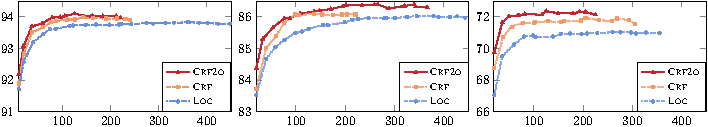
\includegraphics[width=\textwidth]{figures/convergency.pdf}
    \caption{
        Convergence curves (LAS vs. training epochs) on dev data of PTB, CoNLL09, and NLPCC19.
    }
    \label{fig:convergency}
\end{figure*}

\subsection{Main Results}


% 这一段要改写一下。dev只要讲一下,和test规律比较一致即可。

Table~\ref{table:dev-test} lists the main results on the dev and test data.
The trends on dev and test are mostly consistent.
For a fair comparison with previous works, we only consider those without using extra resources such as ELMo \cite{peters-etal-2018-deep} and BERT \cite{devlin-etal-2019-bert}.
We can see that our baseline \textsc{Loc} achieves the best performance on both PTB and CoNLL09.
%is highly competitive.% and achieve state-of-the-art performance.
%We mainly report the results on the test.

%The trends of results on dev are consistency with that on the test, and we ignore the repeat description.
%dev和test趋势类似,说明比较稳定。

On PTB, both \textsc{Crf} and \textsc{Crf2o} fail to improve the parsing accuracy further,
probably because the performance is already very high.
However, as shown by further analysis in Section \ref{section:analysis},
the positive effect is actually introduced by structural learning and high-order modeling.
%英文上性能提高不大,也不显著,我们认为很重要的原因是英文的性能已经很高。

On CoNLL09, \textsc{Crf} significantly outperforms \textsc{Loc},
and \textsc{Crf2o} can further improve the performance.
%CoNLL09上提高更明显一些,CRF显著高于Local,而CRF2O进一步提高。

On the partially annotated NLPCC19 data, \textsc{Crf} outperforms \textsc{Loc} by a very large margin,
indicating the usefulness of structural learning in the scenario of partial annotation.
\textsc{Crf2o} further improves the parsing performance by explicitly modeling second-order subtree features.
These results confirm our intuitions discussed in Section \ref{sub@section:partial-annotation}.
Please note that the parsing accuracy looks very low because the partially annotated tokens
are usually difficult for models.
%with words


%NLPCC19性能很低是因为测试集局部标注最难的。

%NLPCC19上CRF的提高很大,说明structural training很有用,而加入二阶分值后能进一步提高性能;和我们在第x节的讨论很契合。

% Results show that the performance on \textsc{Crf} and \textsc{Crf2o} is very similar with \textsc{Loc} on PTB.
% We believe this is mainly because we build a strong baseline based on biaffine parser, and further adding structural information can't bring additional benefits.
% \textsc{Crf} is slightly better than \textsc{Loc} on CoNLL09 (0.13\%/0.20\%, $p < 0.05$), while \textsc{CrfBib} achieve a more significant ($p < 0.005$) improvement of 0.48\%/0.54\% than \textsc{Crf}.

% Both \textsc{Crf} and \textsc{CrfBib} work well on NLPCC19, which lead to an improvement of 0.42\%/0.67\% and 1.10\%/0.62\% respectively.
% This indicates that structural learning and higher-order information are more useful for partial annotation. We leave detailed analysis in the next section.

% In general, \textsc{Crf2o} can bring significant improvement to the parsing performance over \textsc{Loc}, especially for partial-annotated data.
% Results indicates that our second-order \textsc{Crf}-Based model can achieve very advanced performance and leads to competitive results compared with previous works.

\subsection{Analysis}
\label{section:analysis}

%In this subsection, we try to look deeper into the results for more insights.

\begin{table}[tb!]
    \setlength{\tabcolsep}{5pt}
    \centering
    \begin{tabular}{llccccc}
        \toprule
                                 &                & \multicolumn{3}{c}{SIB} & \multirow{2}{*}{UCM} & \multirow{2}{*}{LCM}                                   \\
                                 &                & P                       & R                    & F                                                      \\[2pt]
        \hline
        \\[-15pt]
        \multirow{3}{*}{PTB}     & \textsc{Loc}   & 91.16                   & 90.80                & 90.98                & 61.59          & 50.66          \\
                                 & \textsc{Crf}   & 91.24                   & 90.92                & 91.08                & 61.92          & 50.33          \\
                                 & \textsc{Crf2o} & \textbf{91.56}          & \textbf{91.11}       & \textbf{91.33}       & \textbf{63.08} & \textbf{50.99} \\[2pt]
        \hline
        \\[-15pt]
        \multirow{3}{*}{CoNLL09} & \textsc{Loc}   & 79.20                   & 79.02                & 79.11                & 40.10          & 28.91          \\
                                 & \textsc{Crf}   & 79.17                   & 79.55                & 79.36                & 40.61          & 29.38          \\
                                 & \textsc{Crf2o} & \textbf{81.00}          & \textbf{80.63}       & \textbf{80.82}       & \textbf{42.53} & \textbf{30.09} \\
        \bottomrule
    \end{tabular}
    \caption{test数据上子树和完全树的结果.}
    \label{table:dev-test-subtree}
\end{table}

%In the following, we conduct detailed analysis on the test data, in order to explore the advantages of structural learning and high-order information.

\paragraph{Impact of MBR decoding.} For \textsc{Crf} and \textsc{Crf2o}, we by default to perform MBR decoding, which employs the Eisner algorithm over marginal probabilities \cite{smith-smith-2007-probabilistic} to find the best tree.
\begin{equation}
    \begin{split}
        & {\boldsymbol{y}}^* = \arg\max_{\boldsymbol{y}} \left[\sum_{i \rightarrow j \in \boldsymbol{y}}{p(i \rightarrow j|\boldsymbol{x})} \right]
    \end{split}
\end{equation}
% against the Maximum A Posteriori (MAP) decoding used in Equation~\ref{equation:map-decoding}
%To measure the impact of MBR decoding, in
Table~\ref{table:dev-test} reports the results of directly finding 1-best trees according to dependency scores. %not using the marginal probabilities.
%From the table, we can clearly see that
Except for PTB, probably due to the high accuracy already, MBR decoding brings small yet consistent improvements for both \textsc{Crf} and \textsc{Crf2o}.
% 传统模型上,MBR decoding的提高也不是特别大。
%almost does not bring any improvement on PTB, and has  on CoNLL09 and NLPCC19.
%These observations are not in line with the conclusion of \citet{smith-smith-2007-probabilistic}, indicating that MBR decoding is not as that useful as previous non-neural works when using deep neural networks like multi-layer BiLSTMs.

\paragraph{Convergence behavior.}

% 我们想观察一下训练过程中dev上性能的变化和收敛速度,来进一步观察不同模型的性能。
% 可以更清晰的看到CRF和CRF2O都能进一步提高模型的性能,而且很稳定。即使英文上最终性能差不多,但是其实从曲线上看,还是有优势的。
% 总的来讲,structural learning和high-order modeling,可以帮助模型提高性能,或者至少能加速收敛(由于loss更多了?前面我写了一段话,应该能用上)
% 两个方面来解释收敛速度变快、编号的原因。loss变多,结构化约束确实能够帮助模型,更有效的得到合适的gradient。哈哈哈!

图~\ref{fig:convergency} compares the convergence curves. % of \textsc{Loc}, \textsc{Crf2o}, and \textsc{Crf}.
For clarity, we plot one data point corresponding to the peak LAS every 20 epochs.
We can clearly see that both structural learning and high-order modeling
consistently improve the model.
\textsc{Crf2o} achieves steadily higher accuracy and converges much faster than the basic \textsc{Loc}.
%Though the final performance is

%We observe that of the three models, the later needs less epochs than the former to converge, and the \textsc{Crf}-based model achieve the peak performance in the very earlier epochs than \textsc{Loc}.
%This shows that when using the structural learning, we are able to achieve higher performance without losing the training efficiency too much.

\paragraph{Performance at sub- and full-tree levels.}

\begin{figure}[tb]
    \centering
    \begin{subfigure}[b]{0.45\textwidth}
        \centering
        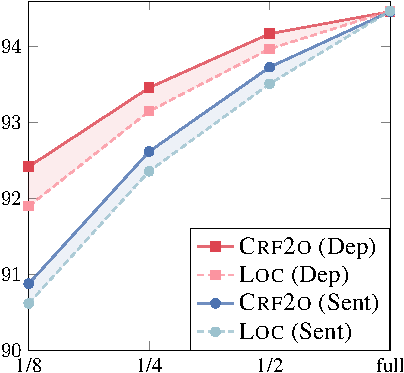
\includegraphics[width=1.\textwidth]{figures/part-gap-ptb.pdf}
    \end{subfigure}
    \begin{subfigure}[b]{0.45\textwidth}
        \centering
        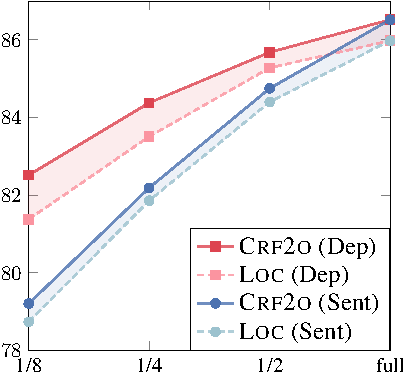
\includegraphics[width=1.\textwidth]{figures/part-gap-conll.pdf}
    \end{subfigure}
    \caption{
        LAS on PTB (left) and CoNLL09-test (right) regarding the amount of training data (dependencies vs. sentences).
    }
    \label{fig:part-gap}
\end{figure}


\begin{table*}[tb]
\setlength{\tabcolsep}{3.4pt}
\centering
\begin{tabular}{lccccccccccccc}
\toprule
& bg & ca & cs & de & en & es & fr & it & nl & no & ro & ru & Avg.\\[1pt]
\hline
\\[-9pt]
\multicolumn{14}{c}{UD2.2} \\[1pt]
% \hline
% \\[-9pt]
$\textsc{Loc}_{\textsc{mst}}$ &         90.44  &         91.11  &         91.04                   &         80.21                   &         86.86                   &         90.67                   &         87.99  &         91.19                    &         88.24                    &         90.35                   &         86.24                    &         93.01                    &         88.95 \\
\textsc{Loc}                  &         90.45  &         91.14  &         90.97                   &         80.02                   &         86.83                   &         90.56                   &         87.76  &         91.14                    &         87.72                    &         90.74                   &         86.20                    &         93.01                    &         88.88 \\
\textsc{Crf}                  &         90.73  &         91.25  &         91.01                   & \textbf{80.56}\rlap{$^\dagger$} &         86.92                   &         90.81\rlap{$^\dagger$}  & \textbf{88.16} &         91.64\rlap{$^\dagger$}   &         88.10                    &         90.85                   &         86.50                    &         93.17\rlap{$^\dagger$}   &         89.14\rlap{$^\ddagger$} \\
\textsc{Crf2o}                & \textbf{90.77} & \textbf{91.29} & \textbf{91.54}\rlap{$^\dagger$} &         80.46                   & \textbf{87.32}\rlap{$^\dagger$} & \textbf{90.86}\rlap{$^\dagger$} &         87.96  & \textbf{91.91}\rlap{$^\ddagger$} & \textbf{88.62}\rlap{$^\ddagger$} & \textbf{91.02}\rlap{$^\dagger$} & \textbf{86.90}\rlap{$^\ddagger$} & \textbf{93.33}\rlap{$^\ddagger$} & \textbf{89.33}\rlap{$^\ddagger$} \\[1pt]
\multicolumn{14}{c}{using raw text} \\[1pt]
Ji19           & 88.28 & 89.90 & 89.85 & 77.09 & 81.16 & 88.93 & 83.73 & 88.91 & 84.82 & 86.33 & 84.44 & 86.62 & 85.83 \\
% \textsc{Crf2o} & \textbf{89.70} & \textbf{90.65} & \textbf{91.06} & \textbf{77.71} & \textbf{82.78} & \textbf{90.26} & \textbf{85.78} & \textbf{90.46} & \textbf{86.30} & \textbf{89.29} & \textbf{85.69} & \textbf{91.97} & \textbf{87.64} \\
\textsc{Crf2o} & \textbf{89.72} & \textbf{91.27} & \textbf{90.94}  & \textbf{78.26} & \textbf{82.88} & \textbf{90.79} & \textbf{86.33} & \textbf{91.02} & \textbf{87.92} & \textbf{90.17} & \textbf{85.71} & \textbf{92.49} & \textbf{88.13} \\
\hline
\\[-9pt]
\multicolumn{14}{c}{UD2.3} \\[1pt]
% \hline
% \\[-9pt]
$\textsc{Loc}_{\textsc{mst}}$   &         90.56  &         91.03  &         91.98  &         81.59  & 86.83 &         90.64  & 88.23 &         91.67  &         88.20  &         90.63  & 86.51 & 93.03 &         89.23 \\
\textsc{Loc}                    &         90.57  &         91.10  &         91.85  &         81.68  & 86.54 &         90.47  & 88.40 &         91.53  &         88.18  &         90.65  & 86.31 & 92.91 &         89.19 \\
\textsc{Crf}   &         90.52  & \textbf{91.19} &         92.02  &         81.43  &         86.88\rlap{$^\dagger$}  &         90.76\rlap{$^\dagger$}  &         88.75  &         91.76  &         88.08  & \textbf{90.79} & 86.54 & 93.16\rlap{$^\ddagger$} &         89.32\rlap{$^\ddagger$} \\
\textsc{Crf2o} & \textbf{90.76} &         91.12  & \textbf{92.15}\rlap{$^\ddagger$} & \textbf{81.94} & \textbf{86.93}\rlap{$^\dagger$} & \textbf{90.81}\rlap{$^\ddagger$} &         \textbf{88.83}\rlap{$^\dagger$}  & \textbf{92.34}\rlap{$^\ddagger$} & \textbf{88.21}\rlap{$^\dagger$} & 90.78 & \textbf{86.62} & \textbf{93.22}\rlap{$^\ddagger$} & \textbf{89.48}\rlap{$^\ddagger$} \\
\multicolumn{14}{c}{using gold POS tags} \\[1pt]
Zhang19        & 90.15 & 91.39 & 91.10 & 83.39 & 88.52 & 90.84 & 88.59 & 92.49 & 88.37 & 92.82 & 84.89 & 93.11 & 89.85 \\
\textsc{Crf2o} & \textbf{91.32} & \textbf{92.57} & \textbf{92.66} & \textbf{84.56} & \textbf{88.98} & \textbf{91.88} & \textbf{89.83} & \textbf{92.94} & \textbf{89.85} & \textbf{93.26} & \textbf{87.39} & \textbf{93.86} & \textbf{90.76} \\
\bottomrule
\end{tabular}
\caption{LAS on UD2.2 and UD2.3 test datasets.
% For fair comparison with \citet{zhang-etal-2019-empirical} (Zhang19), we also report the results of \textsc{Crf2o} that uses gold POS tags.
Again, $\dagger$ and $\ddagger$ means significance level at $p<0.05$ and $p<0.005$ respectively against the \textsc{Loc} parser. }
\label{table:ud2.3-test}
\end{table*}


% \begin{tabular}{ccccc}
% \toprule
% & $\textsc{Local}_{\textsc{mst}}$ & \textsc{Local} & \textsc{Crf} & \textsc{Crf2o} \\
% \hline
% bg   & 90.32 &         90.37  &         90.50                   & \textbf{90.66} \\
% ca   & 90.77 &         90.97  &         91.16\rlap{$^\dagger$}  & \textbf{91.39}\rlap{$^\ddagger$} \\
% cs   & 90.80 &         90.87  & \textbf{91.16}                  &         91.01 \\
% de   & 80.48 &         80.23  &         80.44                   & \textbf{80.52} \\
% en   & 86.87 &         86.93  &         86.84                   & \textbf{87.07} \\
% es   & 90.63 &         90.54  &         90.72\rlap{$^\dagger$}  & \textbf{91.03}\rlap{$^\ddagger$} \\
% fr   & 87.66 &         87.72  &         87.92                   & \textbf{88.36}\rlap{$^\dagger$} \\
% it   & 91.85 & \textbf{91.90} &         91.89                   &         91.83 \\
% nl   & 87.81 &         87.90  &         88.74\rlap{$^\ddagger$} & \textbf{89.04}\rlap{$^\ddagger$} \\
% no   & 90.51 &         90.79  &         90.61                   & \textbf{90.99} \\
% ro   & 86.39 &         86.41  &         86.42                   & \textbf{86.52} \\
% ru   & 93.11 &         93.10  &         93.04                   & \textbf{93.33}\rlap{$^\ddagger$} \\
% \hline
% Avg. & 88.93 &         88.98  &         89.12\rlap{$^\dagger$}   & \textbf{89.31}\rlap{$^\ddagger$} \\
% \bottomrule
% \end{tabular}
% \caption{LAS on CoNLL18-test datasets. Again, $\dagger$ and $\ddagger$ means significance level at $p<0.05$ and $p<0.005$ respectively against the \textsc{Local} parser. %Ji19: \citet{ji-etal-2019-graph}
% }
% \label{table:conll18-gold-test}
% \end{table}


Beyond the dependency-wise accuracy (UAS/LAS), we
would like to evaluate the models regarding performance at sub-tree and full-tree levels.
Table~\ref{table:dev-test-subtree} shows the results. We skip the partially labeled NLPCC19 data.
%虽然整体性能看到了,但是我们想得到更多的insights,by looking deeper.
%To gain more insights on the influence on subtrees, we report the P/R/F value regarding to siblings and UCM/LCM on the test data of PTB and CoNLL09, as shown in Table~\ref{table:dev-test-subtree}. Results of NLPCC19 are ignored since the proper adjacent siblings can't be convinced in the partial-annotated data.
UCM means unlabeled complete matching rate, i.e., the percent of sentences obtaining whole correct skeletal trees, while
LCM further requires that all labels are also correct.


For SIB, we evaluate the model regarding unlabeled adjacent-sibling subtrees % to see the effect of second-order modeling.
(system outputs vs. gold-standard references). % See equation (6) for the definition of an adjacent-sibling subtree. For example,
According to Equation~\ref{eq:score-definition-2o},
$(i,k,j)$ is an adjacent-sibling subtree, if and only if $w_k$ and $w_j$ are both children of $w_i$ at the same side, and there are no other children of $w_i$ between them.
Given two trees, we can collect all adjacent-sibling subtrees and compose two sets of triples.
Then we evaluate the P/R/F values.
Please note that it is impossible to evaluate SIB for partially annotated references.

We can clearly see that by modeling adjacent-sibling subtree scores,
the SIB performance obtains larger improvement than both \textsc{Crf} and \textsc{Loc},
and this further contributes to the large improvement on full-tree matching rates (UCM/LCM).

%Results show that, even the improvement of UAS/LAS on PTB is very modest, there still exists significant difference in the aspect of siblings.
%Specifically, \textsc{Crf2o} achieve a improvement of 0.35\% over \textsc{Loc} on the F-value of siblings.
%It is noted that the results of \textsc{Loc} and \textsc{Crf2o} on UAS/LAS are already distinguishable on CoNLL09, and such gap is further amplified if we look at the sibling structures.

% Moreover, from the global perspective, \textsc{Crf2o} outperforms \textsc{Loc} by 0.59\%/0.16\% and 2.44\%/1.13\% on UCM/LCM of PTB and CoNLL09 respectively.
% This indicates that even if the high-order can't bring more gains in the simple accuracy (UAS), it works much better than \textsc{Loc} from the whole sentence aspect.

\paragraph{Capability to learn from partial trees.}

%为了进一步分析为什么局部标注的NLPCC19性能非常好,我们设计了新的实验。
%In order to further verify that the effectiveness of the \textsc{Crf2o} model
To better understand why \textsc{Crf2o} performs very well on partially annotated NLPCC19,
%in learning from partial trees,
we design more comparative experiments by retaining either a proportion of random training sentences (full trees) or a proportion of random dependencies for each sentence (partial trees).
图~\ref{fig:part-gap} shows the results.
% on PTB-dev and conll09-dev?.
%The curves on conll09 have very similar trends (omitted for saving space).

We can see that the performance gap is quite steady
when we gradually reduce the number of training sentences.
% 其实挺怪的,一般baseline下降的话,会提高大一点的。不知道CoNLL情况如何。
In contrast, the gap clearly becomes larger when each training sentence has less annotated dependencies.
This shows that \textsc{Crf2o} is superior to the basic \textsc{Loc} in
utilizing partial annotated data for model training.
% The results also indicate that: 不是说baseline性能低,second-order就能产生更大的提高。这个是之前的一个错误的直觉。
% in the scenario of partial annotation.
% 此处得根据实验结果进行更新:full annotation下gap比较稳定,而partial annotation情况下gap变大。

%为了进一步验证CRF2O可以更好的从局部标注数据中学习,我们做了一个对比试验。
%一方面是随机删除一部分句子,另一组实验室随机删除句子中的一定比例的弧。



% To clarify in which scenario \textsc{Crf2o} is more useful compared with \textsc{Loc}, we turn the attention to the performance of models trained with partial data of PTB. Concretely, we reduce the training data size in two ways, one is masking the edges randomly to simulate the partial annotation, another is directly choosing a subset from the training data. We depict the trends of performance as the data size changes in 图~\ref{fig:part-gap}.

% As illustrated in the figure, \textsc{Crf2o} does not reflect its advantages compared with \textsc{Loc} if we directly train on a small proportion of the training instances.
% On the contrary, as we discard more edges from the full-annotated data, then the performance between \textsc{Crf2o} and \textsc{Loc} is magnified.
% For example, the difference of LAS on 1/2 annotated PTB is only 0.2\%, while is 0.61\% on 1/16 annotated. We can observe from the figure that the gap between the two models is amplified in proportion to the number of retained edges.

\subsection{Results on Universal Dependencies}

Table~\ref{table:ud2.3-test}
compares different models on UD datasets, which contain a lot of non-projective trees.
% To simplify comparison and significance test, we adopt the gold tokenization setting.
% For ease of comparison, on UD2.2, we follow \citet{ji-etal-2019-graph} and report the results of \textsc{Crf2o} on the test data that auto-segmented on the raw text.
% On UD2.3, we extra use the gold POS tag embeddings for \textsc{Crf2o} and compare it with \citet{zhang-etal-2019-empirical}.
%are kindly shared by
%We directly adopt the data of
%Here, We thank
%for kindly sharing their data,
%including tokenization results (by UDPipe)
% including their multilingual pre-trained word embeddings.
% \citet{ji-etal-2019-graph},
%For the raw text setting under automatic tokenization,
%we use the official evaluation script.
% under two settings, on raw texts with officially provided tokenization (by UDPipe), and on gold-standard tokenization.
%Comparing with the recent results of \citet{ji-etal-2019-graph}, who also adopt the biaffine parser but use POS tag embeddings, we can see that our model is much stronger than theirs. 这句话就不说了。
%Please refer to Section %\ref{section:relwork}
%for detailed discussion.
% Since this work focuses on projective dependency parsing,
We adopt the pseudo-projective approach \cite{nivre-nilsson-2005-pseudo} for handling the ubiquitous non-projective trees of most languages. % with non-projective trees.
Basically, the idea is to transform non-projective trees into projective ones using more complex labels for post-processing recovery.

% % \begin{table}[tbh]
% \setlength{\tabcolsep}{3.5pt}
% \centering
% \begin{tabular}{ccc|ccc}
% \toprule
% & \multicolumn{2}{c|}{Raw} & \multicolumn{3}{c}{Gold} \\
% & Ji19 & \textsc{Crf2o} & \textsc{Local\rlap{$^\ast$}} & \textsc{Loc} & \textsc{Crf2o} \\
% \hline
% bg   & 88.28 & 89.72 & 90.32 & 90.37 & \textbf{90.66} \\
% ca   & 89.90 & 91.27 & 90.77 & 90.97 & \textbf{91.39}\rlap{$^\ddagger$} \\
% cs   & 89.85 & 90.94 & 90.80 & 90.87 & \textbf{91.01} \\
% de   & 81.96 & 78.26 & 80.48 & 80.23 & \textbf{80.52} \\
% en   & 81.16 & 82.88 & 86.87 & 86.93 & \textbf{87.07} \\
% es   & 88.93 & 90.79 & 90.63 & 90.54 & \textbf{91.03}\rlap{$^\ddagger$} \\
% fr   & 83.73 & 86.33 & 87.66 & 87.72 & \textbf{88.36}\rlap{$^\dagger$} \\
% it   & 88.91 & 91.02 & 91.85 & \textbf{91.90} & 91.83 \\
% nl   & 84.82 & 87.92 & 87.81 & 87.90 & \textbf{89.04}\rlap{$^\ddagger$} \\
% no   & 86.33 & 90.17 & 90.51 & 90.79 & \textbf{90.99} \\
% ro   & 84.44 & 85.71 & 86.39 & 86.41 & \textbf{86.52} \\
% ru   & 86.62 & 92.49 & 93.11 & 93.10 & \textbf{93.33}\rlap{$^\ddagger$} \\
% \hline
% Avg. & 86.24 & 88.13 & 88.93 & 88.98 & \textbf{89.31}\rlap{$^\ddagger$} \\
% \bottomrule
% \end{tabular}
% \caption{Results (LAS) on the test data of CoNLL18. Again, $\dagger$ and $\ddagger$ means significance level at $p<0.05$ and $p<0.005$. Ji19: \citet{ji-etal-2019-graph}}
% \label{table:conll18-test}
% \end{table}

% \begin{table}[tbh]
% \setlength{\tabcolsep}{3.5pt}
% \centering

% \begin{tabular}{ccc}
% \toprule
% & \textsc{Local\rlap{$^\ast$}} & \textsc{Loc} & \textsc{Crf2o} \\
% \hline
% bg   & 90.32 & 90.37 & \textbf{90.66} \\
% ca   & 90.77 & 90.97 & \textbf{91.39}\rlap{$^\ddagger$} \\
% cs   & 90.80 & 90.87 & \textbf{91.01} \\
% de   & 80.48 & 80.23 & \textbf{80.52} \\
% en   & 86.87 & 86.93 & \textbf{87.07} \\
% es   & 90.63 & 90.54 & \textbf{91.03}\rlap{$^\ddagger$} \\
% fr   & 87.66 & 87.72 & \textbf{88.36}\rlap{$^\dagger$} \\
% it   & 91.85 & \textbf{91.90} & 91.83 \\
% nl   & 87.81 & 87.90 & \textbf{89.04}\rlap{$^\ddagger$} \\
% no   & 90.51 & 90.79 & \textbf{90.99} \\
% ro   & 86.39 & 86.41 & \textbf{86.52} \\
% ru   & 93.11 & 93.10 & \textbf{93.33}\rlap{$^\ddagger$} \\
% \hline
% Avg. & 88.93 & 88.98 & \textbf{89.31}\rlap{$^\ddagger$} \\
% \bottomrule
% \end{tabular}
% \caption{Results (LAS) on the test data of CoNLL18. Again, $\dagger$ and $\ddagger$ means significance level at $p<0.05$ and $p<0.005$. Ji19: \citet{ji-etal-2019-graph}}
% \label{table:conll18-test}
% \end{table}


\begin{table}[tb]
% \setlength{\tabcolsep}{4.7pt}
\centering

\begin{tabular}{ccccc}
\toprule
& \textsc{Loc} & \textsc{Crf} & \textsc{Crf2o} & Ji19 \\
\hline
bg   & 89.43 &         89.57  & \textbf{89.72} & 88.28 \\
ca   & 90.84 &         91.05  & \textbf{91.27} & 89.90 \\
cs   & 90.79 & \textbf{91.09} &         90.94  & 89.85 \\
de   & 78.13 &         78.30  &         78.26  & 81.96 \\
en   & 82.78 &         82.73  & \textbf{82.88} & 81.16 \\
es   & 90.31 &         90.51  & \textbf{90.79} & 88.93 \\
fr   & 85.68 &         85.59  & \textbf{86.33} & 83.73 \\
it   & 91.17 & \textbf{91.24} &         91.02  & 88.91 \\
nl   & 87.00 &         87.72  & \textbf{87.92} & 84.82 \\
no   & 89.99 &         89.86  & \textbf{90.17} & 86.33 \\
ro   & 85.52 &         85.58  & \textbf{85.71} & 84.44 \\
ru   & 92.10 &         92.17  & \textbf{92.49} & 86.62 \\[1pt]
\hline
\\[-10pt]
Avg. & 87.81 &         87.95  & \textbf{88.13} & 86.24 \\
\bottomrule
\end{tabular}
\caption{LAS on CoNLL18-test datasets.}
\label{table:conll18-test}
\end{table}


%我们在正确分词上对Local和Crf2o进行了比较,
% We then compare different models under the gold tokenization setting.

We can see that for the basic local parsers,
the direct non-projective $\textsc{Loc}_{\textsc{mst}}$ and the pseudo-projective \textsc{Loc}
achieve very similar performance.

More importantly, both \textsc{Crf} and \textsc{Crf2o} produce consistent improvements over the baseline in many languages.
On both UD2.2 and UD2.3, Our proposed \textsc{Crf2o} model achieves the highest accuracy for 10 languages among 12, and obtains significant improvement in more than 7 languages.
Overall, the averaged improvement is 0.45 and 0.29 on UD2.2 and UD2.3 respectively, which is also significant at $p<0.005$.

On average, our \textsc{Crf2o} parser outperforms \citet{ji-etal-2019-graph} by 2.30 on UD2.2 raw texts following CoNLL-2018 shared task setting, and \citet{zhang-etal-2019-empirical} by 0.91 on UD2.3 data with gold POS tags.
It is noteworthy that the German (de) result is kindly provided by Tao Ji after rerunning their parser with predicted XPOS tags, since their reported result in \citet{ji-etal-2019-graph} accidentally used gold-standard sentence segmentation, tokenization, and XPOS tags.
%mainly because we uniformly use CharLSTM in place of POS tags (XPOS in CoNLL18) as input.
%Please note that the unusual result of German (de) reported in \citet{ji-etal-2019-graph}, which is even higher than ours with gold-standard sentence segmentation and tokenization, is caused by using gold POS tags.
% We confirmed this by several communications with the author.
%The new reported result of German in Table~\ref{table:ud2.3-test} is acquired by rerunning their released code.
% 和纪焘交流过了,他正确的结果为77.09,换掉81.96
% 对于Local,pseudo-projective和non-projective的性能相当。
% 在state-of-thart模型的基础上,Crf2o可以提高大部分语言的性能,其中5个语言是显著的。平均而言,也是显著的。
Our \textsc{Crf2o} parser achieves an average LAS of 87.64 using their XPOS tags.

% 另外,我们也和最近的Ji的工作进行了比较,可以看到我们的结果比他们的高很多,说明我们的baseline很强。
% 是否把Raw的结果放在左边?先说Raw,再说Correct Tokenization?

% Finally, we report the LAS on 12 languages selected from CoNLL18, as shown in .
% Considering that there exists a non-negligible proportion of non-projective trees in some languages of CoNLL18, we first convert them to pseudo projective ones and then recover from that using \hyperlink{http://www.maltparser.org/}{MaltParser} \cite{nivre-nilsson-2005-pseudo}.
% Then, the results are two parts.

% First, we report the results of all of our models on the corpora with gold-segmented texts.
% Overall, \textsc{Crf} is slight better than \textsc{Loc} (0.18\%, $p < 0.05$), and \textsc{Crf2o} outperforms \textsc{Loc} by 0.30\% ($p < 0.005$).
% Our model does not improve on some languages like de, it and ro.
% While on some languages like es, fr and nl, the improvements are 0.51\%, 0.74\% and 1.19\%, which are much more obvious.
% All the three models are both trained on converted pseudo projective treebanks, thus we also list the results of the model trained on non-projective trees and decoded by the MST algorithm. Results show that using pseudo projective treebanks is slightly better than non-projective ones.

% Second, for comparison, we compare our best results with previous works and system submissions of CoNLL18 on the auto-segmented data.
% Based on the strong baseline of \textsc{CharLSTM}, our \textsc{Crf2o} outperforms \citet{ji-etal-2019-graph}'s GNN framework by a large margin.
% \textsc{Crf2o} falls behind \citet{che-etal-2018-towards}, which ranks 1st in CoNLL18 shared task,  possibly because of the use of ELMo \cite{peters-etal-2018-deep}.

%这段话明天根据情况进行更新吧。

\section{本章小结}
%本章首先分析了基于模式嵌入的树库转化方法无法充分利用源端树库,其性能受转化数据的一致性的影响很大,具有很强的局限性.
本章分别从树库转化和树库融合两个方面分析了第\ref{sec:super_tc}章中相应方法的缺点. 然后,针对SP-Tree转化方法的低效性和PatEmb转化方法的不稳定性,提出使用Full-Tree转化方法来高效、深度地编码源端树. 接着,本章提出使用语料加权以及合并后微调两种树库融合方法来合理利用含有噪音的转化后源端树库. 最后,在两份双树对齐语料上的实验表明了:
%本章首先指出了第\ref{sec:super_tc}章中树库转化方法和树库融合方法的不足之处.
%然后,针对树库转化任务和树库融合任务提出了一些改进方法,并在两份双树对齐语料上进行实验.
%实验结果表明了:
1)Full-TreeLSTM方法能高效稳定、深度编码源端树信息,并且优于SP-Tree和PatEmb方法;
2)语料加权以及合并后微调的方法可以有效的缓解转化后语料中包含的噪音问题,进一步提升了目标端句法模型性能.
%3)本章提出的改进方法——Full-Tree转化方法和合并后微调的树库融合方法优于第\ref{sec:super_tc}章的SP-Tree转化方法和直接合并的树库融合方法,有效地提升了最终目标端句法模型的性能.
此外,我们在实验中还发现了TreeLSTM输出层的dropout对Full-Tree方法影响较大,合理地设置dropout大小可以获得更高的转化性能.

基于本章研究内容,我们在NLPCC-2019会议(CCF-C类)上发表学术论文一篇.



